% Book pp. 138-150 (PDF pp. 139-151)
\section{Deriving the Equation of a Circle}

The equation of a circle gives information about the centre and radius of the circle.

\begin{center}
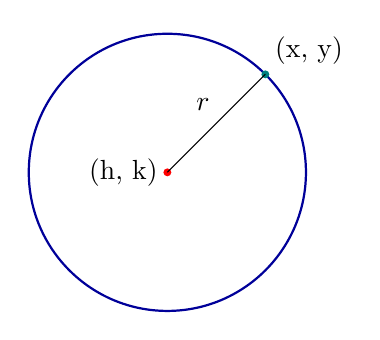
\begin{tikzpicture}[scale=1.1]
  \draw[blue!60!black, thick] (0,0) circle (1.6);
  \fill[red] (0,0) circle (1.3pt);
  \fill[teal] (45:1.6) circle (1.3pt);
  \draw[black] (0,0) -- (45:1.6);
  \node[left] at (0,0) {(h, k)};
  \node[above right] at (45:1.6) {(x, y)};
  \node[above left] at (45:0.85) {$r$};
\end{tikzpicture}
\end{center}
\figcaption{4.6}{A circle}

The equation of a circle with centre (h, k) and radius r is given as:

$(x - h)^2 + (y - k)^2 = r^2$, where $(x, y)$ is any point on the circumference of the
circle.

How did we come by this formula? The following activity will demonstrate.

\begin{activity}{Activity 4.2: Standard Equation of a Circle}
\textbf{Step 1:} Make a copy of the graph below. (a, b) is the centre of the circle and
$(x, y)$ is any point on the circumference of the circle.
\begin{center}
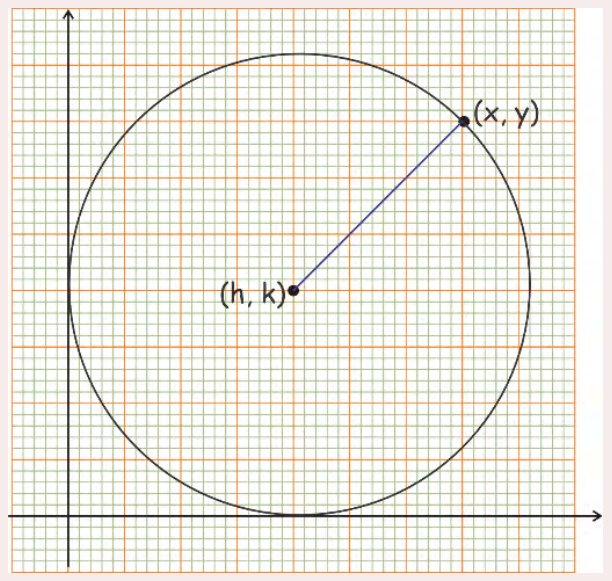
\includegraphics[width=0.45\linewidth]{figures/fig4-7.jpg}
\end{center}
\figcaption{4.7}{Graph of a circle}

\textbf{Step 2:} Using the radius as the hypotenuse, draw a right-angle triangle. Find
its horizontal and vertical distance.

\textbf{Step 3:} Using the Pythagoras theorem, write an equation to connect the
lengths of sides of the triangle.

Your answer should be similar to the one below:
\begin{center}
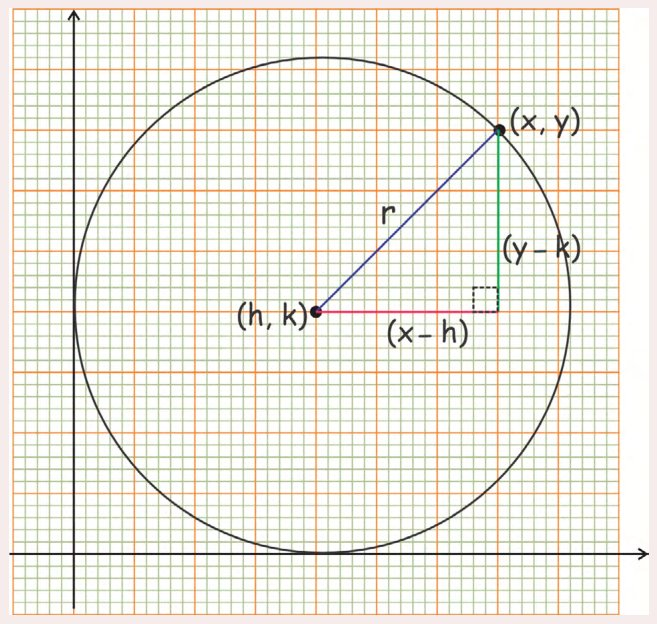
\includegraphics[width=0.48\linewidth]{figures/fig4-8.jpg}
\end{center}
\figcaption{4.8}{Graph of a circle}

From the figure, we have a right-angle triangle with hypotenuse, r, and the
lengths of the other sides as $(x - h)$ and $(y - k)$

Applying Pythagoras theorem, this gives:
\[ \boldsymbol{(x - h)^2 + (y - k)^2 = r^2} \]

Alternatively, you can find the distance between the centre (h, k) and any
point on the circumference (x, y) and you will achieve the same result
\[ r = \sqrt{(x - h)^2 + (y - k)^2} \]
Square both sides of the equation:
\[ \left(r\right)^2 = \left[\sqrt{(x - h)^2 + (y - k)^2}\right]^2 \qquad
   r^2 = (x - h)^2 + (y - k)^2 \]
Rearranging it, we have:
\[ \boldsymbol{(x - h)^2 + (y - k)^2 = r^2} \]
This gives the standard equation of a circle.
\end{activity}

Let us modify this equation for a few special scenarios.

\textbf{Scenario 1}: When the centre of the circle is the origin (0, 0).
\begin{center}
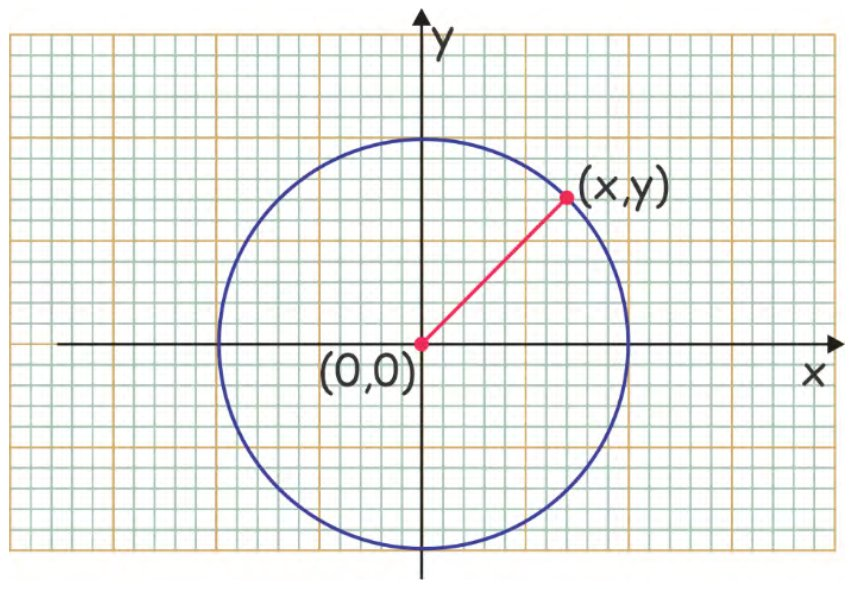
\includegraphics[width=0.6\linewidth]{figures/fig4-9.jpg}
\end{center}
\figcaption{4.9}{Graph of a circle}

When $(h, k) = (0, 0)$, the equation simplifies to:
\begin{align*}
(x - 0)^2 + (y - 0)^2 &= r^2 \\
x^2 + y^2 &= r^2
\end{align*}

\textbf{Scenario 2:} When the centre is any point on the x-axis other than (0, 0).
Remember that on the x-axis, y = 0.
\begin{center}
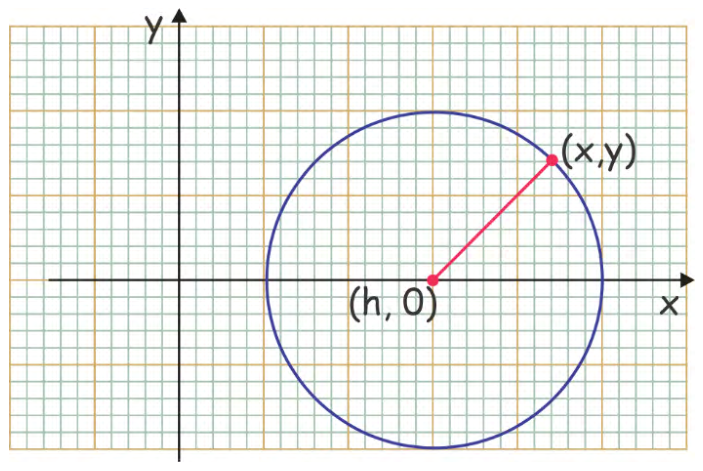
\includegraphics[width=0.5\linewidth]{figures/fig4-10.png}
\end{center}
\figcaption{4.10}{Graph of a circle}

So, we will use $(h, k) = (h, 0)$
\begin{align*}
(x - h)^2 + (y - 0)^2 &= r^2 \\
(x - h)^2 + y^2 &= r^2
\end{align*}

\textbf{Scenario 3:} When the centre is any point on the y-axis other than (o, 0).
Remember that on the y-axis, x=0.
\begin{center}
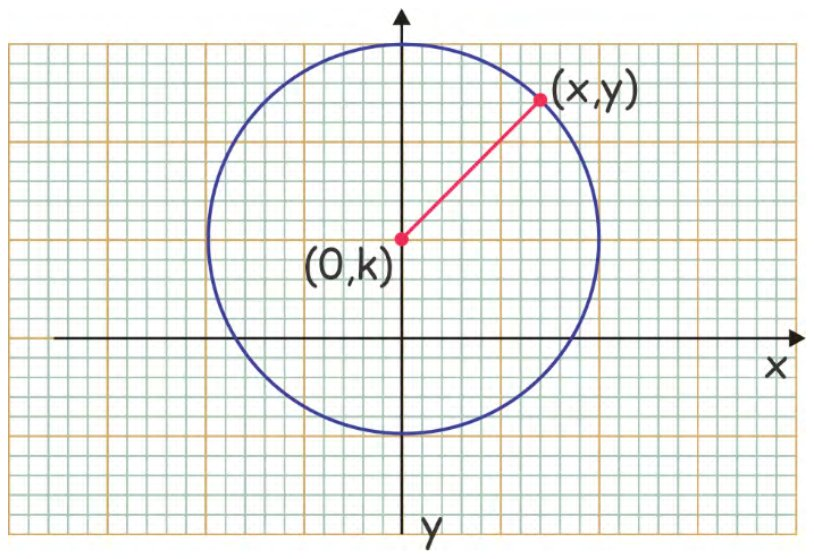
\includegraphics[width=0.55\linewidth]{figures/fig4-11.jpg}
\end{center}
\figcaption{4.11}{Graph of a circle}

So, we will use $(h, k) = (0, k)$
\begin{align*}
(x - 0)^2 + (y - k)^2 &= r^2 \\
x^2 + (y - k)^2 &= r^2
\end{align*}

\begin{example}{Example 4. 2}
Write the standard form of the circle equation with the following properties:
\begin{enumerate}
  \item[a.] Centre (1, 7) and radius 5
  \item[b.] Centre (3, 0) and radius $\frac{2}{3}$
  \item[c.] Centre (0, -5) and radius 2
  \item[d.] Centre (-6, -7) and radius 1
\end{enumerate}

\solution
The standard equation of a circle is given by $(x - h)^2 + (y - k)^2 = r^2$
\begin{enumerate}
  \item[a.] Centre (1, 7) and radius 5\\
  Using the standard equation, replace h with 1, k with 7 and r with 5\\
  $(x - 1)^2 + (y - 7)^2 = 5^2$\\
  $(x - 1)^2 + (y - 7)^2 = 25$
  \item[b.] Centre (3, 0) and radius $\frac{2}{3}$
  \item[c.] using the standard equation, replace h with 3, k with 0 and r with $\frac{2}{3}$
  \item[d.] $(x - 3)^2 + (y - 0)^2 = \left(\frac{2}{3}\right)^2$
  \item[e.] $(x - 3)^2 + y^2 = \frac{4}{9}$
  \item[f.] Centre (0, -5) and radius 2
  \item[g.] $(x - 0)^2 + (y - (-5))^2 = 2^2$
  \item[h.] $x^2 + (y + 5)^2 = 4$
  \item[i.] Centre (-6, -7) and radius 1\\
  $(x - (-6))^2 + (y - (-7))^2 = 1^2$\\
  $(x + 6)^2 + (y + 7)^2 = 1$
\end{enumerate}
\booknote[S4-03]{the solution is lettered a.\ to i.\ in the book: the working of
part (b) is lettered b--e, that of part (c) f--h and that of part (d) i.}
\end{example}

\begin{example}{Example 4.3}
\begin{enumerate}
  \item The diagram shows the graph of circles A, B and C. Use them to answer the
  following questions.
  \begin{center}
  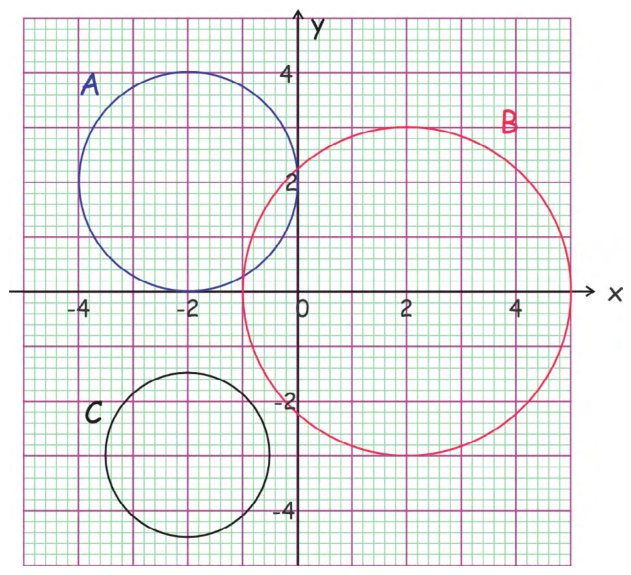
\includegraphics[width=0.5\linewidth]{figures/fig4-12.jpg}
  \end{center}
  \figcaption{4.12}{Graph of circles A, B and C}
  \begin{enumerate}
    \item[a.] Find the diameter of circle:
    \begin{enumerate}
      \item[i.] A
      \item[ii.] B
      \item[iii.] C
    \end{enumerate}
    \item[b.] Write in standard form the equation of:
    \begin{enumerate}
      \item[i.] A
      \item[ii.] B
      \item[iii.] C
    \end{enumerate}
  \end{enumerate}
  \item A phone's WI-FI has a range of 10m in all directions. If the phone is 2m
  West and 5m North, write an equation to represent the area within which the
  phone's Wi-Fi can operate.
\end{enumerate}

\solution
\begin{enumerate}
  \item \textbf{a.}
  \begin{enumerate}
    \item[i.] Diameter of A$=$ 4 units
    \item[ii.] Diameter of B$=$ 6 units
    \item[iii.] Diameter of C$=$ 3 units
  \end{enumerate}
  \textbf{b.}
  \begin{enumerate}
    \item[i.] The coordinates of the centre of circle A is $(-2, 2)$.\\
    Since the diameter is 4 units, it means the radius $= \frac{1}{2} \times 4 = 2$\\
    So, the equation of circle A is: $(x - (-2))^2 + (y - 2)^2 = 2^2$\\
    $(x + 2)^2 + (y - 2)^2 = 4$
    \item[ii.] The coordinates of the centre of circle B is (2, 0).\\
    Since the diameter is 6 units, it means the radius $= \frac{1}{2} \times 6 = 3$\\
    So, the equation of circle B is: $(x - 2)^2 + (y - 0)^2 = 3^2$\\
    $(x - 2)^2 + y^2 = 9$
    \item[iii.] The coordinates of the centre of circle C is $(-2, -3)$.\\
    Since the diameter is 3 units, it means the radius $= \frac{1}{2} \times 3 = \frac{3}{2}$\\
    So, the equation of circle C is: $(x - (-2))^2 + (y - (-3))^2 = \left(\frac{3}{2}\right)^2$\\
    $(x + 2)^2 + (y + 3)^2 = \frac{9}{4}$
  \end{enumerate}
  \item \mbox{}
  \begin{center}
  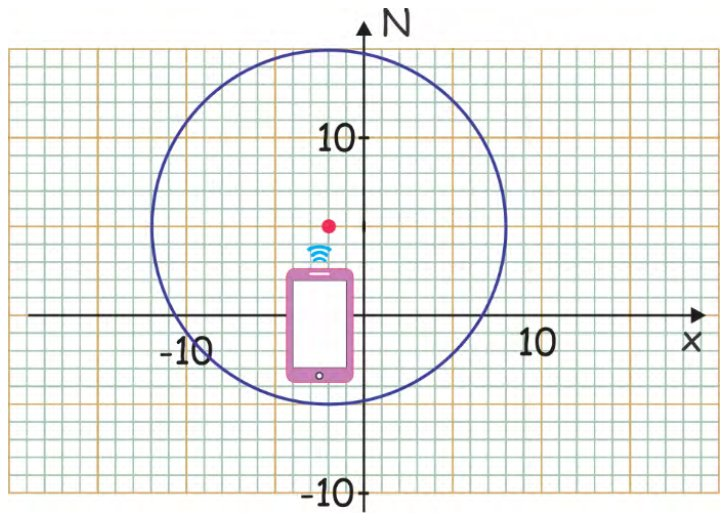
\includegraphics[width=0.55\linewidth]{figures/fig4-13.jpg}
  \end{center}
  \figcaption{4.13}{Graph of the range of the wi-fi signal}

  The range of the wi-fi signal is in the form of a circle with a radius of 10.

  2 units west and 5 units north are the same as the coordinates $(-2, 5)$. This
  point gives the centre of the wi-fi signal.

  The equation of the circle representing the range of the phone's wi-fi signals
  is:\\
  $(x - (-2))^2 + (y - 5)^2 = 10^2$\\
  $(x + 2)^2 + (y - 5)^2 = 100$
\end{enumerate}
\end{example}

\begin{example}{Example 4.4}
A Trotro driver operates within 40km at all angles from a lorry station. The lorry
station is located 15km south and 8km east of the driver's house.
\begin{enumerate}
  \item[a.] Write an equation to represent the driver's travel boundary from the lorry
  station using his house as the origin.
  \item[b.] Find the furthest distance between the driver's house and his travel boundary.
  \item[c.] Find the shortest distance between the driver's house and his travel boundary.
\end{enumerate}

\solution
\begin{center}
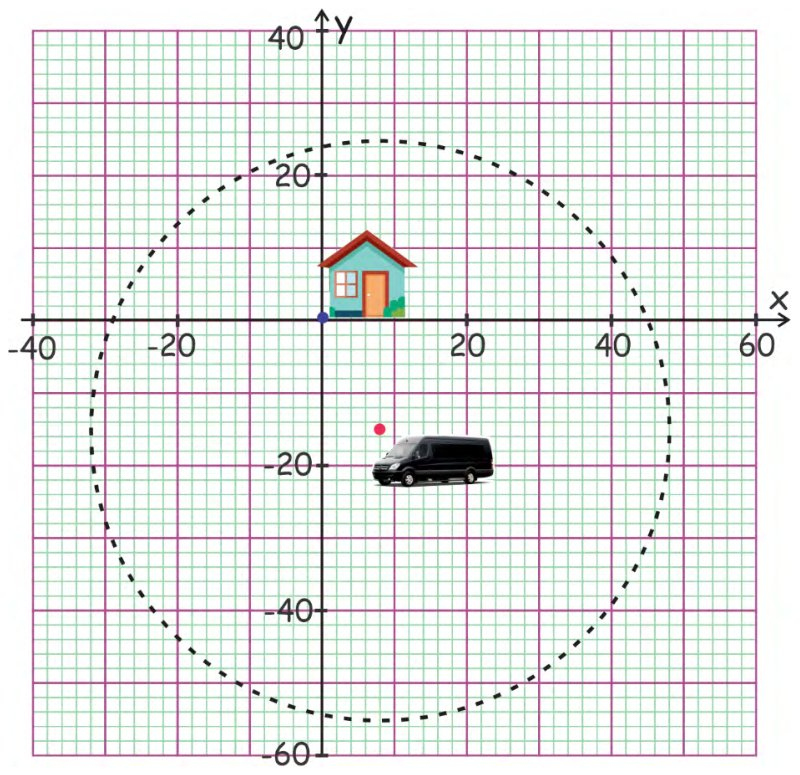
\includegraphics[width=0.6\linewidth]{figures/fig4-14.jpg}
\end{center}
\figcaption{4.14}{Graph of the lorry station and the driver's house}
\begin{enumerate}
  \item[a.] The driver's travel boundary is in the form of a circle with a radius of 40km.
  The centre is the lorry station. From his house, the lorry station is 15km
  south which represents $y = -15$ and 8km east which represents $x = 8$
  \item[b.] Thus, the centre $= (8, -15)$\\
  The equation of the driver's travel boundary is:\\
  $(x - 8)^2 + (y - (-15))^2 = 40^2$\\
  $(x - 8)^2 + (y + 15)^2 = 40^2$
  \item[c.] We first find the distance between the driver's house and the lorry station.
  \begin{align*}
  \text{Distance} &= \sqrt{8^2 + (-15)^2} \\
  &= \sqrt{64 + 225} \\
  &= \sqrt{289} = 17\text{km}
  \end{align*}
  Since his travel distance is 40km, it means the furthest the driver travels
  from his house is 17km $+$40km $=$ \textbf{57km}

  The shortest distance between the driver's house and his travel boundary is
  $40 - 17 = 23$ \textbf{km}
\end{enumerate}
\booknote[S4-04]{the labels b.\ and c.\ are misplaced in the book: ``Thus, the
centre $= (8, -15)$'' and the equation belong to part (a), while the answers to
(b) (57km) and (c) (23 km) both sit under c.}
\end{example}

\subsection{The general equation of a circle}

The general equation of a circle is: $x^2 + y^2 + 2gx + 2fy + c = 0$

To derive this formula, we will modify the standard equation.

We are going to replace the centre $(h, k)$ with $(-g, -f)$.

Recall that the standard equation of a circle is $(x - h)^2 + (y - k)^2 = r^2$ where $(h, k)$
is the centre and $r$ is the radius.

Replacing $(h, k)$ with $(-g, -f)$ we have:
\begin{align*}
(x - (-g))^2 + (y - (-f))^2 &= r^2 \\
(x + g)^2 + (y + f)^2 &= r^2
\end{align*}
Expanding the resulting equation, we get:
\begin{align*}
(x + g)(x + g) + (y + f)(y + f) &= r^2 \\
x^2 + gx + gx + g^2 + y^2 + fy + fy + f^2 &= r^2 \\
x^2 + 2gx + g^2 + y^2 + 2fy + f^2 &= r^2 \\
x^2 + y^2 + 2gx + 2fy + g^2 + f^2 - r^2 &= 0
\end{align*}
Since $g^2 + f^2 - r^2$ will simplify into a constant, replace it with C

This gives,
\[ \boldsymbol{x^2 + y^2 + 2gx + 2fy + c = 0} \]
Note that when the equation is written in the general form,
\begin{align*}
\text{the centre} = (-g, -f) &= \left(\frac{2g}{-2}, \frac{2f}{-2}\right) \\
&= \left(\frac{\textit{Coefficient of } x}{-2}, \frac{\textit{Coefficient of } y}{-2}\right) \\
&= -\frac{1}{2}(\textit{Coefficient of } x, \textit{Coefficient of } y)
\end{align*}
Also, $C = g^2 + f^2 - r^2$. Solving for $r$, we have
\begin{align*}
r^2 &= g^2 + f^2 - c \\
\sqrt{r^2} &= \sqrt{g^2 + f^2 - c} \\
\boldsymbol{r} &= \boldsymbol{\sqrt{g^2 + f^2 - c}}
\end{align*}

\begin{example}{Example 4.5}
Write the general equation of a circle with:
\begin{enumerate}
  \item[a.] Centre (1, 3) and radius 2.
  \item[b.] Centre $(-2, 4)$ and radius $\frac{1}{2}$
\end{enumerate}

\solution
Start from the standard equation and work through it to get the general equation.
\begin{enumerate}
  \item[a.] Centre (1, 3) and radius 2.
  \begin{align*}
  (x - 1)^2 + (y - 3)^2 &= 2^2 \\
  (x - 1)(x - 1) + (y - 3)(y - 3) &= 4 \\
  x^2 - 2x + 1 + y^2 - 6y + 9 &= 4 \\
  x^2 + y^2 - 2x - 6y + 9 + 1 - 4 &= 0 \\
  x^2 + y^2 - 2x - 6y + 6 &= 0
  \end{align*}
\end{enumerate}
Alternatively, we can solve for the variables in the general equation and then
substitute the answer into the general equation.
\begin{align*}
&x^2 + y^2 + 2gx + 2fy + c = 0 \\
&\text{The centre is } = (-g, -f) = (1, 3) \\
&\Longrightarrow g = -1 \text{ and } f = -3 \\
&C = (-1)^2 + (-3)^2 - 2^2 \\
&C = 1 + 9 - 4 \\
&\quad = 6
\end{align*}
Substituting these values into the general equation gives:
\begin{align*}
x^2 + y^2 + 2(-1)x + 2(-3)y + 6 &= 0 \\
x^2 + y^2 - 2x - 6y + 6 &= 0
\end{align*}
\begin{enumerate}
  \item[b.] Centre $(-2, 4)$ and radius $\frac{1}{2}$
  \begin{align*}
  (x - (-2))^2 + (y - 4)^2 &= \left(\frac{1}{2}\right)^2 \\
  (x + 2)(x + 2) + (y - 4)(y - 4) &= \frac{1}{4} \\
  x^2 + 4x + 4 + y^2 - 8y + 16 &= \frac{1}{4} \\
  x^2 + y^2 + 4x - 8y + 20 - \frac{1}{4} &= 0 \\
  x^2 + y^2 + 4x - 8y + \frac{79}{4} &= 0
  \end{align*}
  Multiply through by 4, so we only have integer values:
  \[ 4x^2 + 4y^2 + 16x - 32y + 79 = 0 \]
\end{enumerate}
Alternatively, we can solve for the variables in the general equation and then
substitute the answer into the general equation.
\begin{align*}
&x^2 + y^2 + 2gx + 2fy + c = 0 \\
&\text{The centre is } (-g, -f) = (-2, 4) \\
&\Longrightarrow g = 2 \text{ and } f = -4 \\
&C = (2)^2 + (-4)^2 - \left(\frac{1}{2}\right)^2 \\
&C = 4 + 16 - \frac{1}{4} \\
&C = 20 - \frac{1}{4} = \frac{79}{4}
\end{align*}
Substituting these values into the general equation gives:
\begin{align*}
x^2 + y^2 + 2(2)x + 2(-4)y + \frac{79}{4} &= 0 \\
x^2 + y^2 + 4x - 8y + \frac{79}{4} &= 0
\end{align*}
Multiply through by 4
\[ 4\boldsymbol{x}^2 + 4\boldsymbol{y}^2 + 16\boldsymbol{x} - 32\boldsymbol{y} + 79 = 0 \]
\end{example}

\begin{example}{Example 4.6}
Find the centre and radius of the following circle equations
\begin{enumerate}
  \item[a.] $x^2 + y^2 - 4x - 2y - 4 = 0$
  \item[b.] $x^2 + y^2 - 8x + 6y = 0$
  \item[c.] $x^2 + y^2 + 6x - 40 = 0$
  \item[d.] $4x^2 + 4y^2 - 8x + 3 = 0$
\end{enumerate}

\solution
\begin{enumerate}
  \item[a.] $x^2 + y^2 - 4x - 2y - 4 = 0$

  \textbf{Method 1:} Using completing the square method

  $x^2 - 4x + y^2 - 2y = 4$ group corresponding terms

  $(x^2 - 2x - 2x + 4) + (y^2 - y - y + 1) = 4 + 4 + 1$

  Expand and complete the square
  \begin{align*}
  (x - 2)^2 + (y - 1)^2 &= 9 \\
  (x - 2)^2 + (y - 1)^2 &= 3^2
  \end{align*}
  This shows that the centre is (2, 1) and the radius is 3

  \textbf{Method 2:} Alternatively, compare the given equation to the general equation
  of the circle and solve for the centre and the radius.

  The general equation of a circle is $x^2 + y^2 + 2gx + 2fy + c = 0$

  The given equation is $x^2 + y^2 - 4x - 2y - 4 = 0$

  $x^2 + y^2 + 2(-2)x + 2(-1)y + (-4) = 0$

  By comparing coefficients, we have $g = -2 \Longrightarrow -g = 2$

  Also, $f = -1 \Longrightarrow -f = 1$ and $c = -4$

  Recall that when the circle equation is written in the general form, the centre
  is $(-g, -f)$

  Therefore, the centre is (2, 1).

  You will achieve the same result if you divide the coefficient of $x$ and $y$ by $-2$

  Centre $= (-4 \_\, -2, -2 \_\, -2) = (2, 1)$
  \booknote[S4-05]{the division signs are printed as underscores; read
  $(-4 \div -2,\ -2 \div -2)$.}

  Radius $= r = \sqrt{g^2 + f^2 - c}$

  $r = \sqrt{2^2 + 1^2 - (-4)} = \sqrt{9} = 3$

  \item[b.] $x^2 + y^2 - 8x + 6y = 0$

  \textit{Method 1}: Using the completing the square method, we have:
  \begin{align*}
  x^2 - 8x + 16 + y^2 + 6y + 9 &= 16 + 9 \\
  (x - 4)^2 + (y + 3)^2 &= 25 \\
  (x - 4)^2 + (y + 3)^2 &= 5^2
  \end{align*}
  Therefore, the centre is (4, -3) and the radius is 5

  \textbf{Method 2:} Alternatively, we can re-write the equation as

  $x^2 + y^2 + 2(-4)x + 2(3)y + 0 = 0$

  Comparing this equation to $x^2 + y^2 + 2gx + 2fy + c = 0$, we have:

  $g = -4 \Longrightarrow -g = 4$, $f = 3 \Longrightarrow -f = -3$ and C$=0$

  Therefore, the centre is (4, -3)

  Radius $= r = \sqrt{(-4)^2 + 3^2 - 0} = \sqrt{25} = 5$

  \item[c.] $x^2 + y^2 + 6x - 40 = 0$

  \textbf{Method 1:} Completing the square, we have:
  \begin{align*}
  x^2 + 6x + 9 + y^2 + 2(0)x + 0 &= 40 + 9 + 0 \\
  (x + 3)^2 + (y + 0)^2 &= 49 \\
  (x + 3)^2 + (y + 0)^2 &= 7^2
  \end{align*}
  Centre is (-3, 0) and radius is 7

  \textbf{Method 2:} Alternatively, we can re-write the equation as

  $x^2 + y^2 + 2(3)x + 2(0)y - 40 = 0$

  Comparing this equation to $x^2 + y^2 + 2gx + 2fy + c = 0$, we have:

  $g = 3 \Longrightarrow -g = -3$, $f = 0 \Longrightarrow -f = 0$ and C$= -40$

  Therefore, the centre is (-3, 0)

  Radius $= r = \sqrt{(3)^2 + 0^2 - (-40)} = \sqrt{49} = 7$

  \item[d.] $4x^2 + 4y^2 - 8x + 3 = 0$

  Method 1: Completing the square, we will first divide the equation by 4

  $x^2 + y^2 - 2x + \frac{3}{4} = 0 \quad x^2 - 2x + 1 + y^2 + 0 = -\frac{3}{4} + 1 + 0$

  $(x - 1)^2 + (y + 0)^2 = 1 \_\, 4$

  $\left(x - 1\right)^2 + \left(y + 0\right)^2 = \left(\frac{1}{2}\right)^2$
  \booknote[S4-06]{two equations are run together on one line, and the right-hand
  side of the next line is printed ``$1 \_\, 4$'' for $\frac{1}{4}$.}

  Centre is (1, 0) and radius is $\frac{1}{2}$

  \textbf{Method 2:} Alternatively, we can re-write the equation as:

  $x^2 + y^2 + 2(-1)x + 2(0)y + \frac{3}{4} = 0$

  Comparing this equation to $x^2 + y^2 + 2gx + 2fy + c = 0$, we have:

  $g = -1 \Longrightarrow -g = 1$, $f = 0 \Longrightarrow -f = 0$ and C$= \frac{3}{4}$

  Therefore, the centre is (1, 0)

  Radius $= r = \sqrt{(-1)^2 + 0^2 - \frac{3}{4}} = \sqrt{\frac{1}{4}} = \frac{1}{2}$
\end{enumerate}
\end{example}
